%% SECTION HEADER /////////////////////////////////////////////////////////////////////////////////////
\section{Damage indices}
\label{sec:di}

%% SECTION CONTENT ////////////////////////////////////////////////////////////////////////////////////
In the dissertation, four damage indices are analysed in the time - domain. All of them are considered in two options, the entire length of the signal and the first wave package arrived at the sensor.
The packaged is extracted by windowing the full-length signals of the sensor  with a flattened Gaussian window in the form:
\begin{eqnarray}
	g(t)= \mathrm{exp}\left(-\left(\frac{t-t_0}{w_g}\right) ^{n}\right),
	\label{eq:psi_g}
\end{eqnarray}
where \(t_0\) is the center and \(w_g=0.5N_c/f_c\) is a half-width of the window, and n determines the slope of the window.
Due to the linearity of the models, analysis in the frequency domain was omitted, expecting comparable results as in the time domain.

The following time-domain indices are take into consideration: \ac{p2p}, \ac{rmsd}, \ac{eng} of the signal in two kind.

\begin{eqnarray}
		\mathrm{P2P} & = & \left[\mathrm{max}(\Psi(t)) - \mathrm{min}(\Psi(t))\right] - \left[\mathrm{max}(\Psi_0(t)) - \mathrm{min}(\Psi_0(t))\right],\\
		\mathrm{RMSD} & = & \sqrt{\int{\left[\Psi(t)-\Psi_0(t)\right]^2\diff 		t/\int{\left[\Psi_0(t)\right]^2\diff t}}},\\
		\mathrm{ENG^1} & = & \left(\int{\left[\Psi(t)\right]^2\diff t}-\int{\left[\Psi_0(t)\right]^2\diff t}\right) /\int{\left[\Psi(t)\right]^2\diff t},\\
		\mathrm{ENG^2} & = & \int{\left[\Psi(t)-\Psi_0(t)\right]^2\diff 	t}/\int{\left[\Psi(t)\right]^2\diff t},\\
\end{eqnarray}
where \(\Psi_0(t)\) and \(\Psi(t)\) are the time-domain baseline
signal and the comparison signal registered by sensor, respectively.
The \ac{p2p} is based on the difference between peak-to-peak amplitudes of the monitored and the baseline state.
The \ac{rmsd} measures the error between two states, \ac{eng}\(^1\) compares the difference of the sensor responses energy, and \ac{eng}\(^2\) measures the energy of the signals obtained by the difference of the signals.

The experimental obtained \acp{di} based on the full-length signals are shown in Figs. \ref{fig:DI_exp_full} for the frequency 50, 100 and 150 kHz. 
It can be observed from the figures that the \ac{eng}\(^1\) index is useless as the values are almost constant throughout the damage size range.
In the case of \ac{p2p} index, the values decrease monotonically only for 100 kHz.
In the case of 50 and 150 kHz, the index increases for minor defects and reaches the maximum of around 70 mm of the damage size, after which it begins to decrease.
The best results for damage size analysis were obtained for the \ac{rmsd} and \ac{eng}\(^2\) indices, as the values increase monotonically over the full range of the damage size for each frequency.
The most significant changes are observed at 50 kHz and the smallest at 150 kHz.
 \ref{fig:DI_exp_win}.
\begin{figure}[!tbh]
	\begin{center}
		\includegraphics{Chapter_7/DI_EXP_full}
	\end{center}
	\caption{Experimentally obtained \acp{di} based on full-length signals.}
	\label{fig:DI_exp_full}
\end{figure}

The experimental obtained \acp{di} based on the windowed signals are shown in Figs. \ref{fig:DI_exp_win} for the frequency 50, 100 150 kHz.
The characteristics of all indices are consistent with the related indices determined for the full-length signals.
However, the values of the \ac{rmsd} and \ac{eng}\(^2\) of windowed signals are five and 30 times, respectively, lower than in the case of the entire signals. It is because the extracted signal is an S0 package whose dominant displacements are in-plane.
Consequently, a smaller portion of the energy of the S0 leak into the core in the pristine region. In the case of the full-length response, the \ac{a0} is registered, which dominant displacements are out of the plate, making this mode more sensible for damage like disbonds or delamination.
\begin{figure}[!tbh]
	\begin{center}
		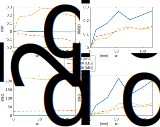
\includegraphics{Chapter_7/DI_EXP_win}
	\end{center}
	\caption{Experimentally obtained \acp{di} based on windowed signals.}
	\label{fig:DI_exp_win}
\end{figure}
\begin{figure}[!tbh]
	\begin{center}
		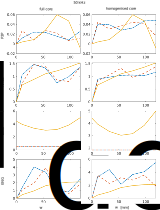
\includegraphics{Chapter_7/DI_F_F_H_50kHz}
	\end{center}
	\caption{\acp{di} based on full-length 50 kHz signals for full core and homogenised model, solid line for experimental measurements, dash-dot line for the model with removed cells, dashed line for the model with removed interface.}
	\label{fig:DI_num_full_50}
\end{figure}
\begin{figure}[!tbh]
	\begin{center}
		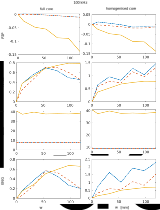
\includegraphics{Chapter_7/DI_F_F_H_100kHz}
	\end{center}
	\caption{\acp{di} based on full-length 100 kHz signals for full core and homogenised model, solid line for experimental measurements, dash-dot line for the model with removed cells, dashed line for the model with removed interface.}
	\label{fig:DI_num_full_100}
\end{figure}
\begin{figure}[!tbh]
	\begin{center}
		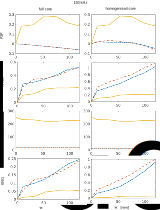
\includegraphics{Chapter_7/DI_F_F_H_150kHz}
	\end{center}
	\caption{\acp{di} based on full-length 150 kHz signals for full core and homogenised model, solid line for experimental measurements, dash-dot line for the model with removed cells, dashed line for the model with removed interface.}
	\label{fig:DI_num_full_150}
\end{figure}
The numerically obtained \acp{di} based on the full-length signals are shown in Figs. \ref{fig:DI_num_full_50} for 50 kHz, \ref{fig:DI_num_full_100} for 100 kHz and \ref{fig:DI_num_full_150} for 150 kHz.
According to the simulation results, similarly to the experimental ones, the \ac{p2p} and \ac{eng}\(^1\) indices show the most inferior useful significance.
In the case of the full core model, no significant differences are observed in the designated indices for damage modelled by removing cells and the interface.
In comparison, more considerable differences for both defect models are visible in the case of the homogenised model.

The numerically obtained \acp{di} based on the windowed signals are shown in Figs. \ref{fig:DI_num_win_50} for 50 kHz, \ref{fig:DI_num_win_100} for 100 kHz and \ref{fig:DI_num_win_150} for 150 kHz.
In this case also the values of the indicators decrease as for the experimental results, except for the \ac{rmsd} 50 kHz.
\begin{figure}[!tbh]
	\begin{center}
		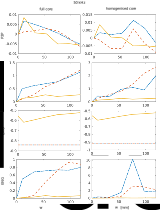
\includegraphics{Chapter_7/DI_W_F_H_50kHz}
	\end{center}
	\caption{\acp{di} based on windowed 50 kHz signals for full core and homogenised model, solid line for experimental measurements, dash-dot line for the model with removed cells, dashed line for the model with removed interface.}
	\label{fig:DI_num_win_50}
\end{figure}
\begin{figure}[!tbh]
	\begin{center}
		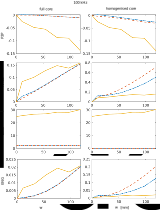
\includegraphics{Chapter_7/DI_W_F_H_100kHz}
	\end{center}
	\caption{\acp{di} based on windowed 100 kHz signals for full core and homogenised model, solid line for experimental measurements, dash-dot line for the model with removed cells, dashed line for the model with removed interface.}
	\label{fig:DI_num_win_100}
\end{figure}
\begin{figure}[!tbh]
	\begin{center}
		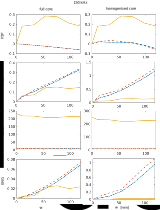
\includegraphics{Chapter_7/DI_W_F_H_150kHz}
	\end{center}
	\caption{\acp{di} based on windowed 150 kHz signals for full core and homogenised model, solid line for experimental measurements, dash-dot line for the model with removed cells, dashed line for the model with removed interface.}
	\label{fig:DI_num_win_150}
\end{figure}
